\chapter{Results}
  The final ray tracer is available at \url{http://github.com/Nemo157/Raytracer}.

  Figure \ref{example} below shows a low quality ten minute render.  As can be
  seen from this image ten minutes isn't long enough to get a very good image.
  The render time is very dependent on image complexity as well as quality, Fig.
  \ref{example2} below was rendered at a similar quality level with slightly
  more anti-aliasing but because of the increased complexity took 4.5X as long.
  As an example of the sort of quality it is possible to get see Figures
  \ref{good-render},\ref{good-render2}, these however took much much longer to
  generate.  This would be OK if you are just trying to get a static high
  quality image.

  \begin{figure}[p]
    \centering
    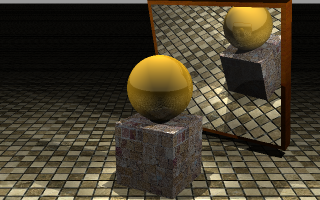
\includegraphics{images/example.png}
    \caption{An example 10 minute render image\label{example}}
  \end{figure}

  \begin{figure}[p]
    \centering
    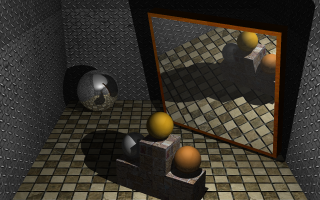
\includegraphics{images/example2.png}
    \caption{An example 46 minute render image\label{example2}}
  \end{figure}

  \begin{figure}[p]
    \centering
    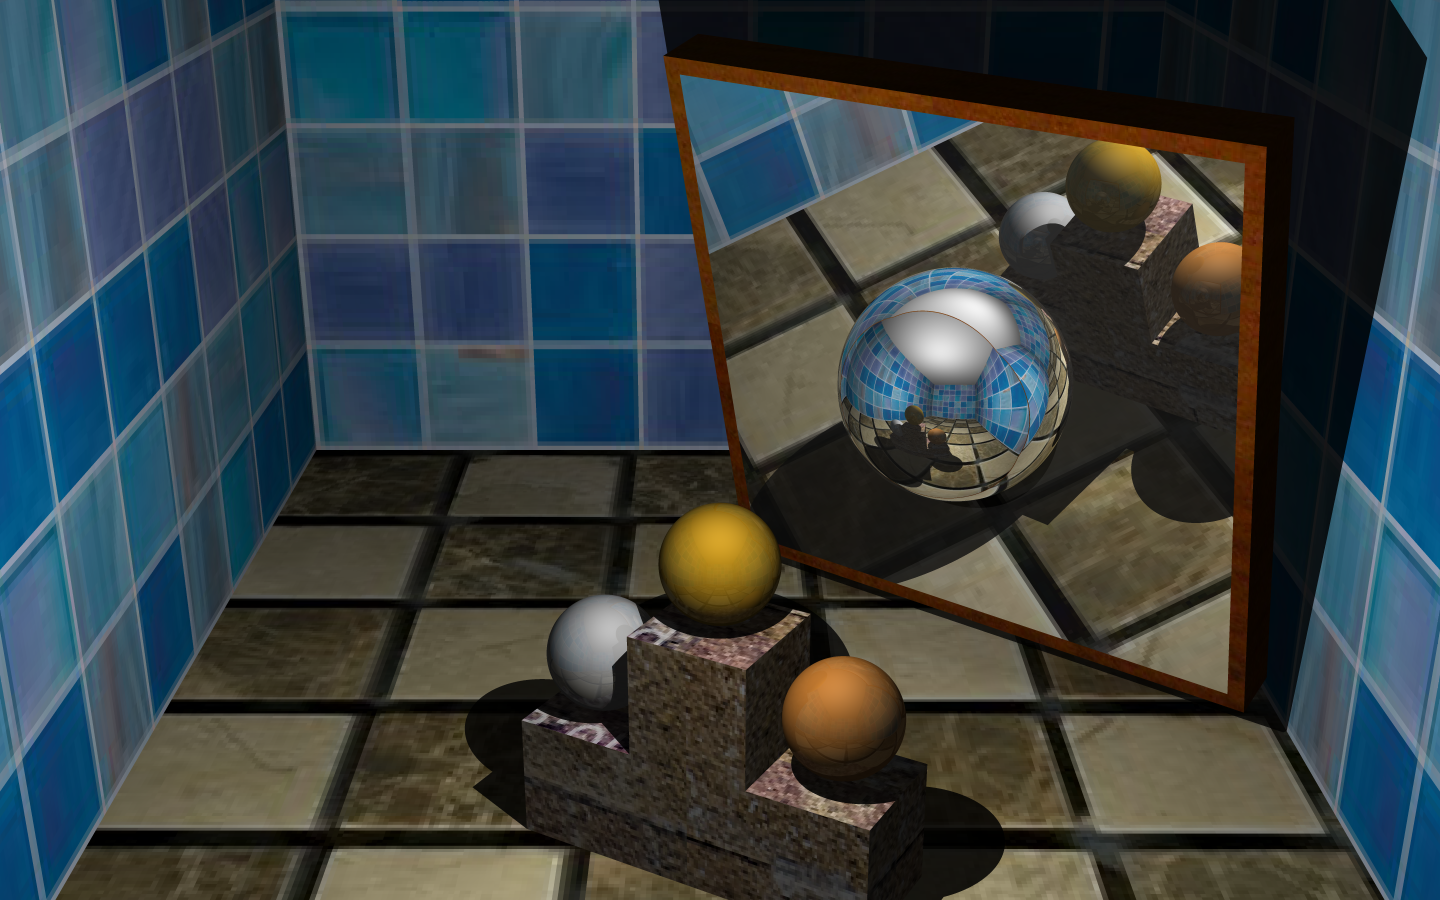
\includegraphics[height=0.9\textwidth,angle=90]{images/image1.png}
    \caption{An 18 hour 31 minute render.\label{good-render}}
  \end{figure}


  \begin{figure}[p]
    \centering
    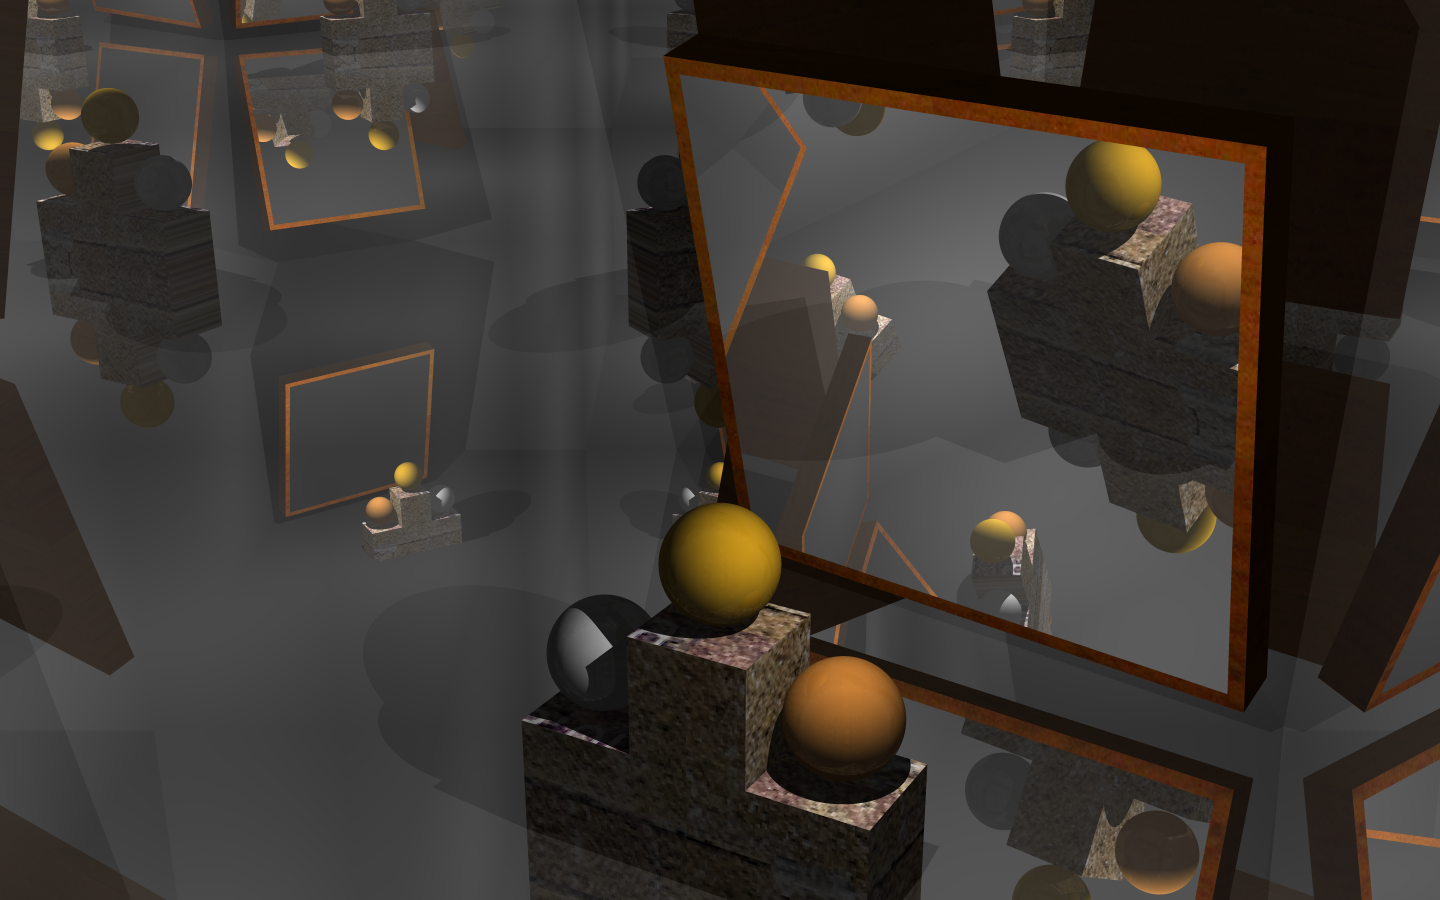
\includegraphics[height=0.9\textwidth,angle=90]{images/image2.png}
    \caption{A 28 hour 43 minute render. Similar scene to above with
             the reflective sphere removed and walls, floor and roof changed to
             reflective surfaces.  Only 5 iterations of reflections are
             calculated.\label{good-render2}}
  \end{figure}
